% figures/ex_type2.tex

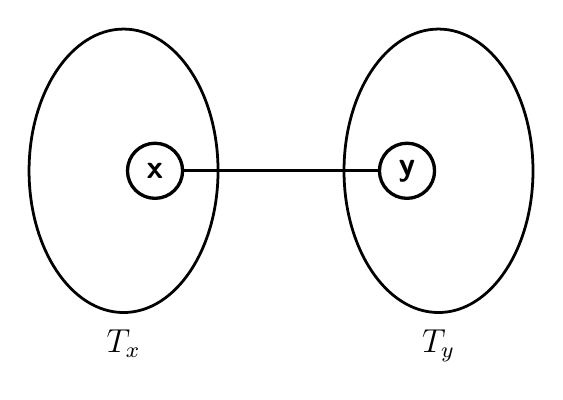
\begin{tikzpicture}[
    % Style for the vertices with labels inside
    vNode/.style={
        circle, 
        draw=black, 
        fill=white, 
        very thick, 
        inner sep=0pt, 
        minimum size=7mm, % Size adjusted for text
        font=\sffamily\bfseries\large
    },
    % Style for the set labels (Tx and Ty)
    setLabel/.style={
        font=\sffamily\bfseries\large,
        anchor=north
    },
    % Style for the edge
    edgeStyle/.style={
        draw=black, 
        line width=1pt
    },
    % Style for the container ellipses
    ellipseStyle/.style={
        draw=black, 
        line width=1pt
    }
]

    % --- COORDINATES ---
    \def\spacing{4} % Slightly wider spacing for the larger nodes

    % --- LEFT COMPONENT (Tx) ---
    \draw[ellipseStyle] (0,0) ellipse (1.2cm and 1.8cm);
    \node[vNode] (Vx) at (0.4, 0) {x};
    \node[setLabel] at (0, -1.9) {$T_x$};

    % --- RIGHT COMPONENT (Ty) ---
    \draw[ellipseStyle] (\spacing,0) ellipse (1.2cm and 1.8cm);
    \node[vNode] (Vy) at (\spacing-0.4, 0) {y};
    \node[setLabel] at (\spacing, -1.9) {$T_y$};

    % --- EDGE ---
    \draw[edgeStyle] (Vx) -- (Vy);

\end{tikzpicture}